%!TEX root = ../thesis.tex

%%%%% Chapter: System Architecture %%%%%
\chapter{System Architecture}
\label{chap:sys-architecture}

\ifpdf
    \graphicspath{{Chapter3/Figs/Raster/}{Chapter3/Figs/PDF/}{Chapter3/Figs/}}
\else
    \graphicspath{{Chapter3/Figs/Vector/}{Chapter3/Figs/}}
\fi


%%% Overview %%%
\section{Overview}

\Cref{fig:sys-diagram-full} shows the system architecture design. The system consists of three subsystems: the OCR engine, the speech recogniser and the core alignment algorithm.

\begin{figure}[!ht]
  \centering
  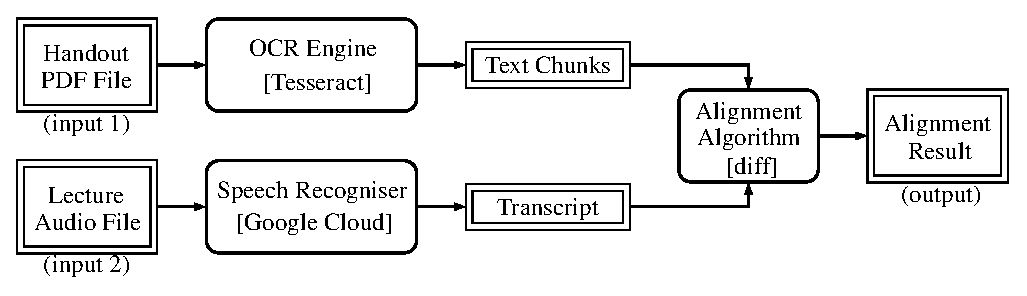
\includegraphics[width=0.95\textwidth]{sys-diagram-full.eps}
  \caption{Diagram of the software system architecture}
  \label{fig:sys-diagram-full}
\end{figure}

% how the system works
The handout PDF file and the corresponding audio file are first fed into the OCR engine and the speech recogniser respectively. The core alignment algorithm accepts the outputs from both the OCR engine and the speech recogniser, and then computes the final alignment result.

% some intuitions
The idea of the system design is that both the handout file and the lecture audio file can be converted to large text strings, which are much simpler to manipulate compared to image and audio data. The speech recogniser is used to produce transcript from the lecture audio file, since in \Cref{sec:intro-aims} we have already stated that the alignment system is based on speech recognition. OCR engine is the most straightforward tool to convert scanned documents to machine-encoded text, so it is also used in the system. The final alignment result could be computed by a suitable algorithm which compares the two large text strings.

% following sections
The following sections will introduce each subsystem in turn. For each subsystem, the general knowledge of the subsystem will be described first, followed by the introduction of the specific tool selected for that subsystem.

%%% OCR engine %%%
\section{OCR Engine}

\subsection{General Introduction}

An OCR (Optical Character Recognition) engine converts the visual representation of text (images) to machine-encoded text (e.g Unicode text). The OCR engine in the system reads the input handout file and extracts textual information within it, which could then be used by the core alignment algorithm.

For most of the publicly available OCR engines, only image files (e.g PNG, JPEG, TIFF) are accepted as inputs, rather than PDF files. Therefore, additional processing which converts the PDF file to a sequence of images is needed before feeding the input to the actual OCR engine. 

In the standard OCR pipeline, there is a Page Layout Analysis (PLA) step which analyses the document layout and identifies distinct blocks of text in the document. The PLA step could be operated at different scales, which in turn produces different levels of bounding-boxes (e.g words, lines, paragraphs). The bounding-boxes are considered to be the `chunks' of the handout which are taken as the input of the core alignment algorithm.

A good OCR engine should be able to recognise printed text of various fonts with high accuracy. Recognition of handwritten text is clearly harder due to the uncertainty of the writing style, however the ability of recognising handwritten text is still desirable since handwritten text is of great interest in the project. Also, the Page Layout Analysis (PLA) of the OCR engine should be as accurate as possible.

\subsection{Selected Tool: Tesseract OCR}
\label{sec:sys-arch-tess}

Tesseract OCR is an open-source command-line OCR engine sponsored by Google since 2006. It is able to perform PLA which finds bounding-boxes of texts at 5 different levels (word, line, paragraph, block, page). The current software system uses Tesseract 4.0 (the recent stable version), which includes an LSTM-based neural network model (pre-trained with 400000 textlines spanning around 4500 fonts), which provides higher recognition accuracy compared to previous versions. The engine could also be fine-tuned or retrained using additional data.

The reason for choosing Tesseract OCR is that it is an open-source command-line tool whose internal model can be fine-tuned or retrained from scratch. Open-source means it's free to use, and command-line tool means that it can be easily integrated into our software system. In addition, it would be possible to improve the accuracy of recognising handwritten text by fine-tuning the Tesseract with additional labelled handwritten dataset.


%%% Speech Recogniser %%%
\section{Speech Recogniser}

\subsection{General Introduction}

A speech recogniser converts human speeches (audio files) to machine-encoded text (e.g Unicode text). Speech recognisers can be trained to recognise different languages (English, Chinese, etc.) in different contexts (math lectures, president speeches, etc.). The output of the speech recogniser is also called the `transcript' of the input audio file.

Different speech recognisers may require different digital format of the input audio file. Usually speech recognisers would prefer the original (uncompressed) audio formats like WAV, or lossless compressed audio formats like FLAC (Free Lossless Audio Codec). However, the input format requirement should not be an issue since there are lots of free audio transcoders available for use.

The output of the speech recogniser is a machine-encoded text string which is also named as the `transcript'. The transcript is usually segmented based on the long pauses in the input speech, and each of the segments is usually associated with a confidence score and a timestamp as in the original audio file. Optionally, timestamps for each word could also be provided in addition to the segment-level timestamps.

The Word Error Rate (WER) is a common measure of the performances of speech recognisers. A good speech recogniser should have a WER as low as possible. It would also be desirable if a speech recogniser can have consistent recognition accuracy in as many different contexts as possible.

\subsection{Selected Tool: Google Cloud Speech-to-Text API}

The current system uses the Google Cloud Speech-to-Text API as the speech recogniser. For long audio files like lecture audio files (typically an hour), the transcription process for the Google Cloud is done asynchronously: the client sends a request to the Google Cloud server; the server processes the input audio data (usually takes 5-10 minutes); the server sends back the transcription result to the client. The API supports most of the mainstream languages including Python, C\# and Java.

The transcription result is a list of segments, each of which contains the transcribed text and its starting timestamp. The timestamp for each individual recognised word is also included in the returned result.

Transcribing an hour-long lecture will generally take a long time if we use offline speech recognisers on our local PC machines. Therefore, using cloud-based speech recognisers would be preferred since they have access to much more computing power and can significantly reduce the transcription time. 

An example lecture has been transcribed using Google Cloud and its WER is roughly 15\%. Since this is a reasonable accuracy and it's hard to find other speech-to-text systems which have the same level of functionality and accuracy, the Google Cloud is selected as the speech recogniser of the current system.


%%% Alignment Algorithm
\section{Alignment Algorithm}

\subsection{General Introduction}

The alignment algorithm finds the correspondence between handout chunks and audio segments, based on the textual outputs from the OCR engine and the speech recogniser. This is the core system part which determines the mappings between the handout and the corresponding audio file. 

As \Cref{fig:sys-diagram-full} shows, the two outputs from the OCR engine and the speech recogniser becomes the two inputs of the alignment algorithm. Both inputs are essentially just segmented text strings: the extracted handout text is segmented by the bounding-boxes and the audio file is segmented into shorter text strings based on the pauses in the speech.

The alignment output is simply just the system output, which has been explained in \Cref{sec:assume-align-res}. Each chunk (bounding-box) of the handout should be mapped to a starting time and an ending time as in the associated audio file. 

\subsection{Selected Tool: Word-based \texttt{diff}}

The \texttt{diff} utility is originally a Unix command-line tool which calcuates and displays the differences between two files. The \texttt{diff} algorithm essentially solves the longest common subsequence (LCS) problem between two sequences of items. For either sequence, those items which are not in the LCS indicate occurrences of differences compared to the other sequence.

In the word-based \texttt{diff} algorithm, the items in the two input sequences should all be words. The use of word-based \texttt{diff} algorithm in the current system is inspired by \cite{lanchantin2015development}, which used a \texttt{diff}-based algorithm to align imperfect captions with audio of TV shows. Based on the previous assumption that the lecturers will read and explain the handouts in strictly sequential order, the word-based \texttt{diff} algorithm could be used to produce acceptable alignment results by finding word matches between the handouts and the lecture audio files. 



\nomenclature[z-PLA]{PLA}{Page Layout Analysis}
\nomenclature[z-WER]{WER}{Word Error Rate}
\nomenclature[z-API]{API}{Application Programming Interface}
\nomenclature[z-LCS]{LCS}{Longest Common Subsequence}


%% example of a nice-looking table
% \begin{table}
% \caption{Even better looking table using booktabs}
% \centering
% \label{table:good_table}
% \begin{tabular}{l c c c c}
% \toprule
% \multirow{2}{*}{Dental measurement} & \multicolumn{2}{c}{Species I} & \multicolumn{2}{c}{Species II} \\ 
% \cmidrule{2-5}
%   & mean & SD  & mean & SD  \\ 
% \midrule
% I1MD & 6.23 & 0.91 & 5.2  & 0.7  \\

% I1LL & 7.48 & 0.56 & 8.7  & 0.71 \\

% I2MD & 3.99 & 0.63 & 4.22 & 0.54 \\

% I2LL & 6.81 & 0.02 & 6.66 & 0.01 \\

% CMD & 13.47 & 0.09 & 10.55 & 0.05 \\

% CBL & 11.88 & 0.05 & 13.11 & 0.04\\ 
% \bottomrule
% \end{tabular}
% \end{table}
